\documentclass[12pt]{article}

\usepackage{setspace}
\usepackage[top=1in, bottom=1in, left=1in, right=1in]{geometry}
\usepackage{lipsum}
\usepackage{graphicx}

\title{Evaluation of Nonparametric Classification Methods for Predicting Fake News from Article Titles}
\author{Nathaniel Hawkins}
\date{}

\begin{document}
	\maketitle
	
	\section{Introduction}
	
	
	
	\section{Methods}
	
	\lipsum[2]
	
	\section{Data}

    %% Begin Table Summarizing Dataset
    \begin{table}
    \begin{center}
        \begin{tabular}{|c|c|}
            \hline
            \textbf{Number of Article Titles}&44,266\\
            \hline
            \textbf{Number of Article Titles (True)}&21,416\\
            \hline
            \textbf{Number of Article Titles (Fake)}&22,850\\
            \hline
            \textbf{Mean Length of Titles (Words)}&9.29\\
            \hline
            \textbf{Median Length of Titles (Words)}&9\\
            \hline
            \textbf{Minimum Length of Titles (Words)}&1\\
            \hline
            \textbf{Maximum Length of Titles (Words)}&29\\
            \hline
            \textbf{Number of Features After One-Hot Encoding}&18,206\\
            \hline
        \end{tabular}
        \caption{Summary of dataset used in this work. Lengths shown in this table are the texts following preprocessing.}
        \label{table:1}
    \end{center}  
    \end{table} 	
    
     %% Histogram of title lengths
    \begin{figure}[htbp]
        \centerline{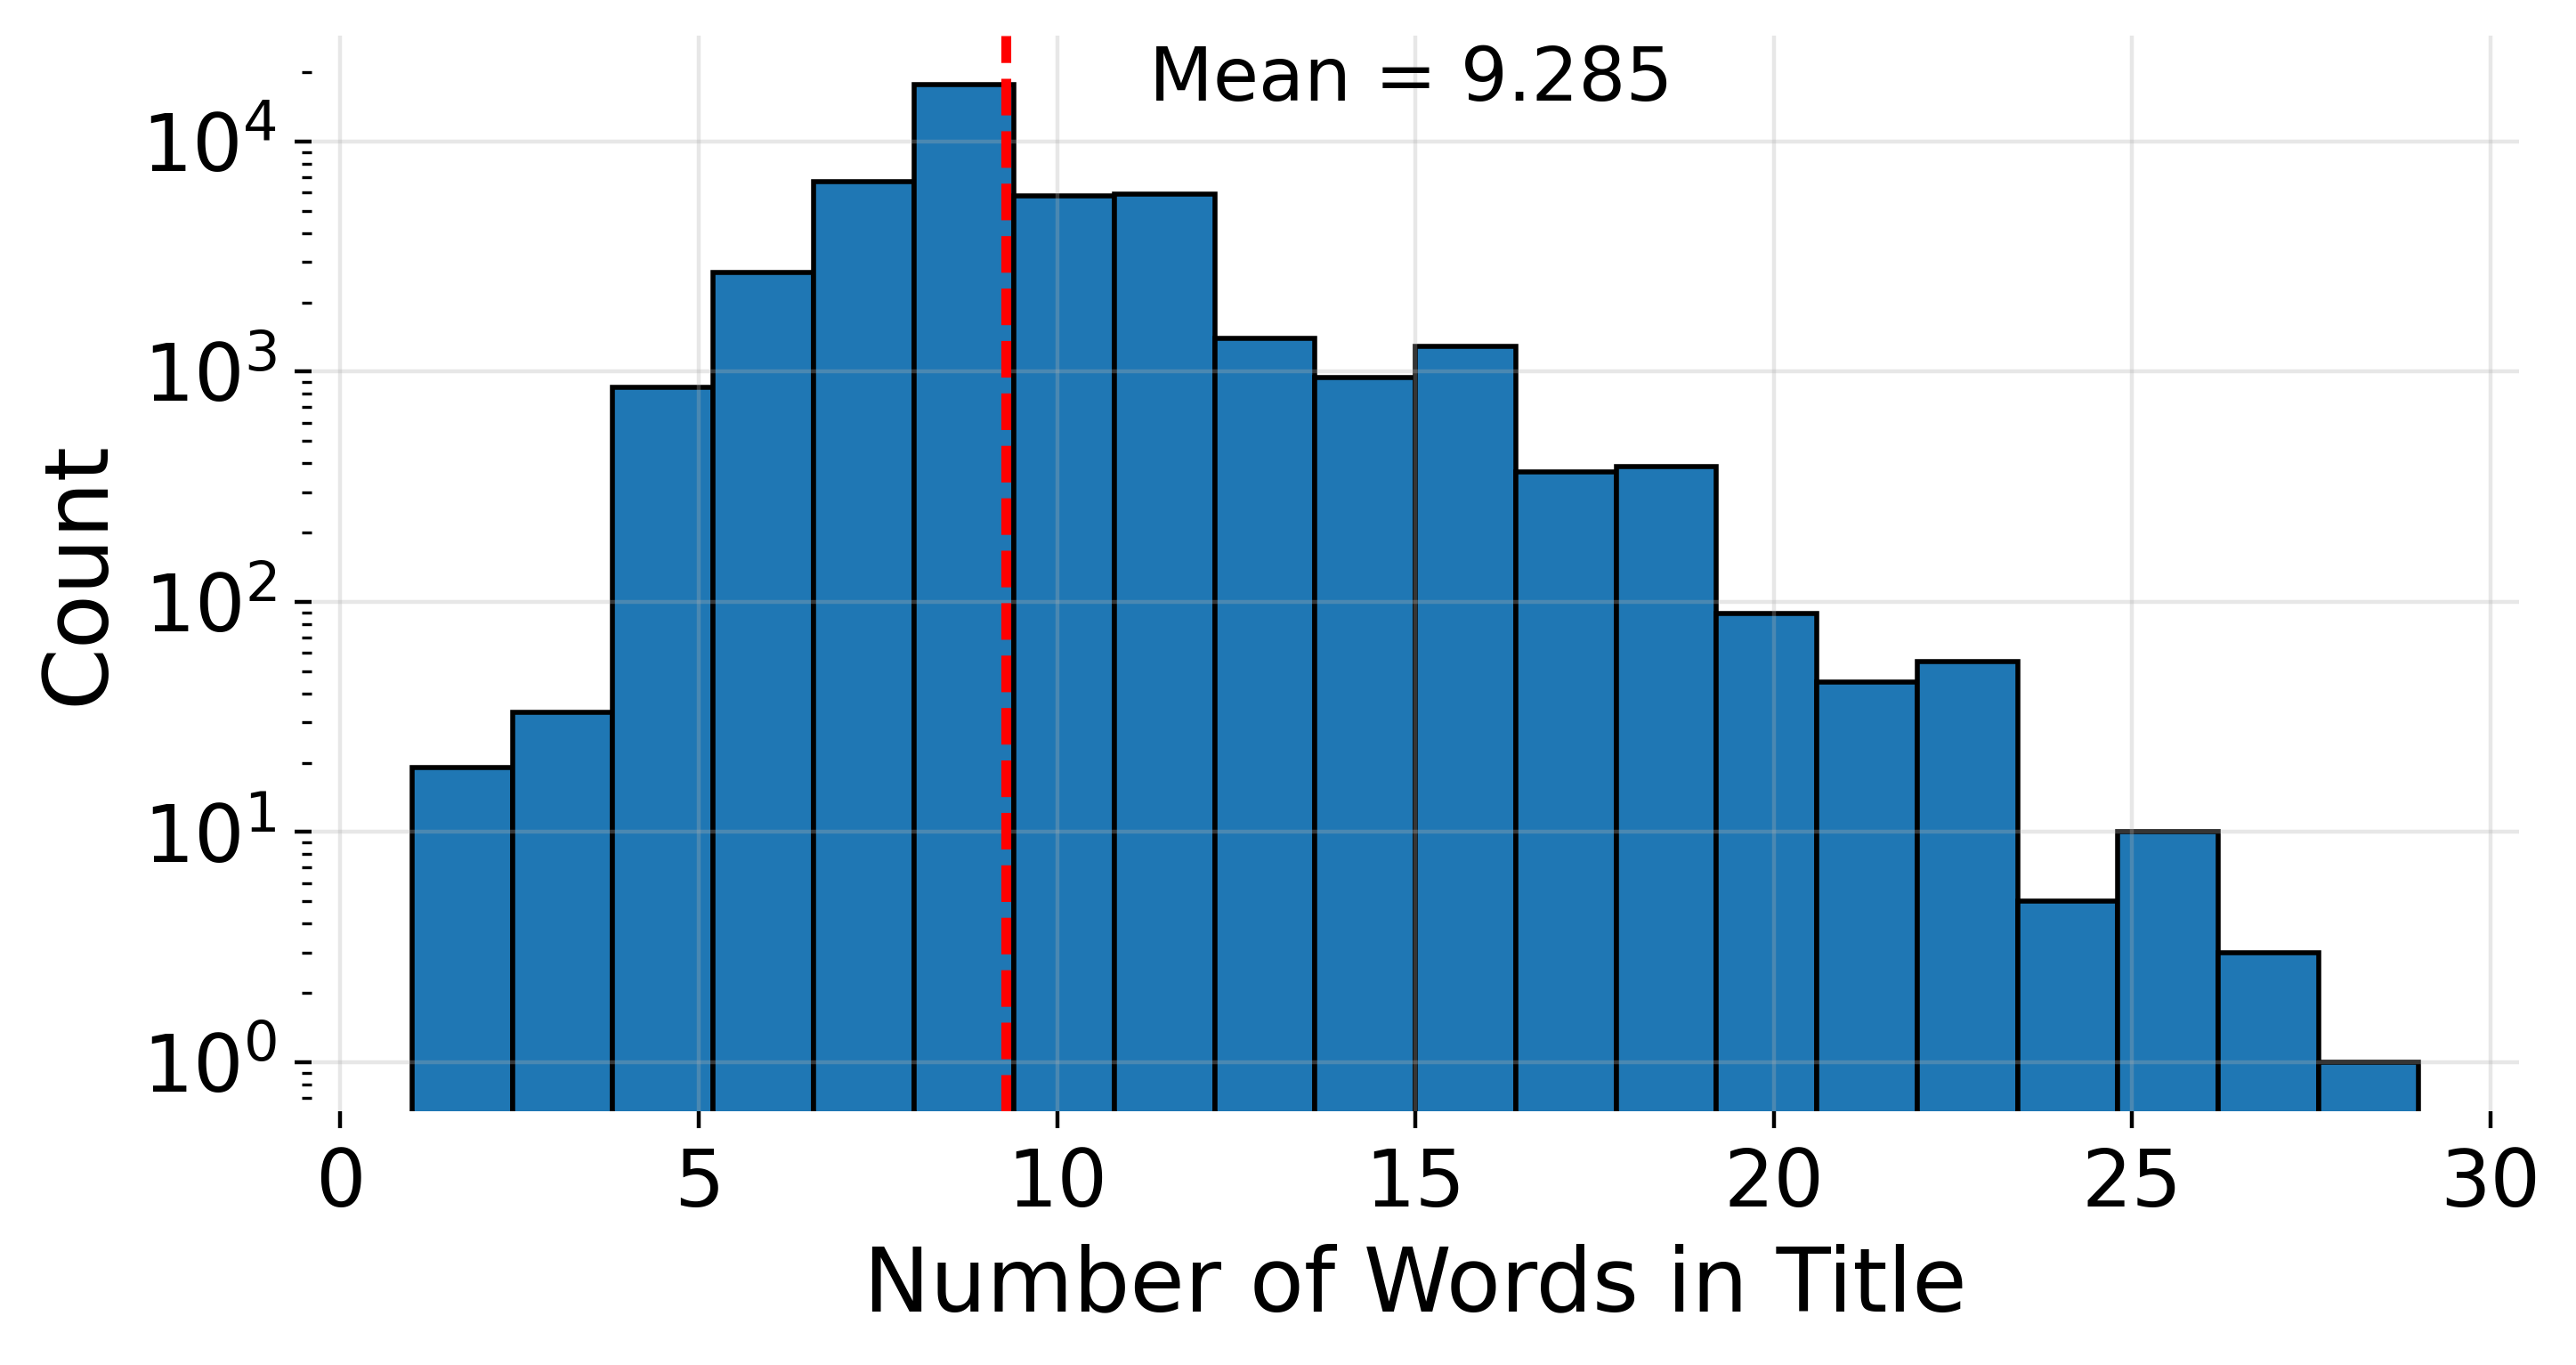
\includegraphics[scale=1]{../results/length_of_description.png}}
        \caption{Histogram of length of article titles. Mean description shown with verticle red line. Y-axis is logarithmically scaled.}
        \label{fig:1}
\end{figure}

	\section{Results}
	
    \lipsum[4]	
	
	\section{Discussion and Conclusions}
	
    \lipsum[5]	
    
    
    %% Bibliography
    \newpage
    \nocite{*}
    \bibliography{report} 
    \bibliographystyle{ieeetr}
	
\end{document}